\documentclass[12pt]{article}

%Bibliography   
    \usepackage{apacite}
    \bibliographystyle{apacite}
    %http://www.ctan.org/tex-archive/biblio/bibtex/contrib/apacite/apacite.pdf
 
%Essay Header
	\pagestyle{myheadings}
	\markright{\hfill \emph{Horowitz }}

%pdfLaTeX: TeX Gyre Termes
	%\usepackage{tgtermes}
	\usepackage[T1]{fontenc}

%Sectioning
    \usepackage{sectsty}
    \sectionfont{\fontsize{13}{15}\selectfont}

%Packages
    \usepackage[margin=1in]{geometry}
    \usepackage{setspace}
    \usepackage[leftmargin = 1in, rightmargin = 0in, vskip = 0in]{quoting}
    \usepackage{microtype}




\usepackage{centernot}

\newtoggle{professormode}
%\toggletrue{professormode} %STUDENTS: DELETE or COMMENT this line



\title{MATH 390.4 Spring 2020 Homework \#2}

\author{Tziporah Horowitz} %STUDENTS: write your name here

\iftoggle{professormode}{
\date{Due 11:59PM Monday KY604, February 24, 2020 \\ \vspace{0.5cm} \small (this document last updated \currenttime~on \today)}
}

\renewcommand{\abstractname}{Instructions and Philosophy}

\begin{document}
\maketitle

\iftoggle{professormode}{
\begin{abstract}
The path to success in this class is to do many problems. Unlike other courses, exclusively doing reading(s) will not help. Coming to lecture is akin to watching workout videos; thinking about and solving problems on your own is the actual ``working out.''  Feel free to \qu{work out} with others; \textbf{I want you to work on this in groups.}

Reading is still \textit{required}. For this homework set, read the first chapter of \qu{Learning from Data} and Chapter 2 of Silver's book. Of course, you should be googling and reading about all the concepts introduced in class online. This is your responsibility to supplement in-class with your own readings.

The problems below are color coded: \ingreen{green} problems are considered \textit{easy} and marked \qu{[easy]}; \inorange{yellow} problems are considered \textit{intermediate} and marked \qu{[harder]}, \inred{red} problems are considered \textit{difficult} and marked \qu{[difficult]} and \inpurple{purple} problems are extra credit. The \textit{easy} problems are intended to be ``giveaways'' if you went to class. Do as much as you can of the others; I expect you to at least attempt the \textit{difficult} problems. 

This homework is worth 100 points but the point distribution will not be determined until after the due date. See syllabus for the policy on late homework.

Up to 7 points are given as a bonus if the homework is typed using \LaTeX. Links to instaling \LaTeX~and program for compiling \LaTeX~is found on the syllabus. You are encouraged to use \url{overleaf.com}. If you are handing in homework this way, read the comments in the code; there are two lines to comment out and you should replace my name with yours and write your section. The easiest way to use overleaf is to copy the raw text from hwxx.tex and preamble.tex into two new overleaf tex files with the same name. If you are asked to make drawings, you can take a picture of your handwritten drawing and insert them as figures or leave space using the \qu{$\backslash$vspace} command and draw them in after printing or attach them stapled.

The document is available with spaces for you to write your answers. If not using \LaTeX, print this document \textit{including this first page} and write in your answers. \inred{I do not accept homeworks which are \textit{not} on this printout.}

\end{abstract}

\thispagestyle{empty}
\vspace{1cm}
NAME: \line(1,0){380}
\clearpage
}

\section{Silver's Book, Chapter 2}


\begin{enumerate}

\intermediatesubproblem{If one's goal is to fit a model for a phenomenon $y$, what is the difference between the approaches of the hedgehog and the fox? Answer using notation from class (i.e. $t ,f, g, h^*, \delta, \epsilon, e, t, z_1, \ldots, z_t, \mathbb{D}, \mathcal{H}, \mathcal{A}, \mathcal{X}, \mathcal{Y}, X, y, n, p, x_{\cdot 1}, \ldots, x_{\cdot p}, x_{1 \cdot}, \ldots, x_{n \cdot}$, etc.). Connecting this to the modeling framework should really make you think about what Tetlock's observation means for political and historical phenomena.
\ans 
Foxes are better at prediction than hedgehogs because they improve as more information becomes available. Hedgehogs only believe in one hypothesis set, $\mathcal{H}$, while foxes will adjust their hypotheses based on the $x$'s observed.
}

\easysubproblem{Why did Harry Truman like hedgehogs? Are there a lot of people that think this way?
\ans 
Truman believed that foxes were too uncertain with their answers. Like many others, Truman liked bold predictions.
}


\hardsubproblem{Why is it that the more education one acquires, the less accurate one's predictions become?
\ans 
The more information a hedgehog acquires, the faster he can attribute it toward a prediction.
}


\easysubproblem{Why are probabilistic classifiers (i.e. algorithms that output functions that return probabilities) better than vanilla classifiers (i.e. algorithms that only return the class label)? We will move in this direction in class soon.
\ans
Probabilistic classifiers are better than vanilla classifiers because they give an almost definite prediction of the percentage of correct outcomes, rather than an objective prediction that has a higher likelihood of being wrong.
}

\end{enumerate}

\pagebreak

\section{The SVM}

\begin{enumerate}

\easysubproblem{State the hypothesis set $\mathcal{H}$ inputted into the support vector machine algorithm. Is it different than the $\mathcal{H}$ used for $\mathcal{A}$ = perceptron learning algorithm?
\ans The SVM's hypothesis set differs from the perceptron's hypothesis set by a factor of $b$:
\begin{align*}
    \mathcal{H} = \big\{ \indic{\vec{w} \cdot \vec{x} + b \geq 0 } : \vec{w} \in \mathbb{R}^p, b \in \mathbb{R} \big\}
\end{align*}
}

\hardsubproblem{[MA] Prove the SVM converges. State all assumptions. Write it on a separate page.}\spc{0}

\hardsubproblem{Let $\mathcal{Y} = \braces{-1,1}$. Rederive the cost function whose minimization yields the SVM line in the linearly separable case. 
\ans
\begin{align*}
    l_a :\ \ \forall y_i = 1,\ \ \ \ \ \ \vec{w} \cdot \vec{x_i} - (b+1) &\geq 0 \\
    \vec{w} \cdot \vec{x_i} - b &\geq 1 \\
    y_i(\vec{w} \cdot \vec{x_i} - b) &\geq y_i = 1 \\
     l_b :\ \ \forall y_i = -1,\ \ \ \vec{w} \cdot \vec{x_i} - (b-1) &\leq 0 \\
     \vec{w} \cdot \vec{x_i} - b &\leq -1 \\
     -y_i(\vec{w} \cdot \vec{x_i} - b) &\leq y_i = -1 \\
     y_i(\vec{w} \cdot \vec{x_i} - b) &\geq 1
\end{align*}
\begin{align*}
    l: \ \ \text{maximize } \frac{2}{||\vec{w}||} \text{ such that } y_i(\vec{w} \cdot \vec{x_i} - b) &\geq 1
\end{align*}
}

\easysubproblem{Given your answer to (c) rederive the cost function using the \qu{soft margin} i.e. the hinge loss plus the term with the hyperparameter $\lambda$. This is marked easy since there is just one change from the expression given in class.
\ans
\begin{align*}
    Cost = {\argmin_\limits{\vec{w} \in \mathbb{R}^p, b \in \mathbb{R}} } \bigg\{ \frac{1}{n} \text{max} \big\{ 0, 1-y_i(\vec{w} \cdot \vec{x_i} - b) \big\} + \lambda ||\vec{w}||^2 \bigg\}
\end{align*}
}

\end{enumerate}

\pagebreak

\section{The k Nearest Neighbors (KNN) Algorithm}

\begin{enumerate}

\easysubproblem{Describe how the algorithm works. Is $k$ a \qu{hyperparameter}?
\ans For $\vec{x^*}$, find $x_{i_{(1)}}, \ldots, x_{i_{(k)}}$ where the distances $d(\vec{x^*}, \vec{x_{i_{(k)}}})$ are the $k$ smallest and let $\hat{y} = mode[y_{i_{(1)}}, \ldots, y_{i_{(k)}}]$. $k$ is a hyperparameter.
}

\hardsubproblem{Assuming $\mathcal{A} = $ KNN, describe the input $\mathcal{H}$ as best as you can.
\ans $\mathcal{H}$ is defined by a distance metric and the hyperparameter, $k$.
}

\hardsubproblem{When predicting on $\mathbb{D}$ with $k=1$, why should there be zero error? Is this a good estimate of future error when new data comes in? (Error in the future is called \emph{generalization error} and we will be discussing this later in the semester).
\ans When $k=1$, the error will be $0$ because $\vec{x^*}$ will be mapped to itself. However, it is not a good estimate for future error because a datapoint that was not previously observed will not be able to map to itself.
}

\end{enumerate}

\section{The Linear Model with $p=1$}

\begin{enumerate}

\easysubproblem{What does $\mathbb{D}$ look like in the linear model with $p=1$? What is $\mathcal{X}$? What is $\mathcal{Y}$?
\ans 
\begin{align*}
    \mathbb{D} &= \begin{Bmatrix}
        \begin{bmatrix}
            1 & x_1 \\
            \vdots & \vdots \\
            1 & x_n
        \end{bmatrix} &
        \begin{bmatrix}
            y_1 \\
            \vdots \\
            y_n
        \end{bmatrix}
    \end{Bmatrix} \\ \\
    \mathcal{X} &= \mathbb{R}^{n \times (p+1)} \\
    \mathcal{Y} &= \mathbb{R}^n
\end{align*}
}


\easysubproblem{Consider the line fit using the ordinary least squares (OLS) algorithm. Prove that the point $<\xbar, \ybar>$ is on this line. Use the formulas we derived in class.
\ans
\begin{align*}
    g(x) &= b_0 + b_1x \\
    b_1 &= r\frac{s_y}{s_x} \\
    b_0 &= \ybar - b_1\xbar \\
    &= \ybar - \xbar r\frac{s_y}{s_x} \\
    g(\xbar) &= \ybar - \xbar r\frac{s_y}{s_x} + \xbar r\frac{s_y}{s_x} = \ybar
\end{align*}
}

\intermediatesubproblem{Consider the line fit using OLS. Prove that the average prediction $\hat{y}_i := g(x_i)$ for $x_i \in \mathbb{D}$ is $\ybar$.
\ans 
\begin{align*}
    \oneover{n} \sum_{i=1}^n \hat{y}_i &= \oneover{n} \sum_{i=1}^n (b_0 + b_1x_i) \\
    &= b_0 + \frac{b_1}{n} \sum_{i=1}^n x_i \\
    &= b_0 + b_1\xbar \\
    &= \ybar
\end{align*}
}


\intermediatesubproblem{Consider the line fit using OLS. Prove that the average residual $e_i$ is 0 over $\mathbb{D}$.
\ans
\begin{align*}
    \oneover{n}\sum_{i=1}^n e_i &= \oneover{n}\sum_{i=1}^n (y_i - \hat{y}_i) \\
    &= \ybar - \oneover{n}\sum_{i=1}^n \hat{y}_i \\
    &= \ybar - \oneover{n}\sum_{i=1}^n (b_0 + b_1x_i) \\
    &= \ybar - \ybar \\
    &= 0
\end{align*}
}

\intermediatesubproblem{Why is the RMSE usually a better indicator of predictive performance than $R^2$? Discuss in English.
\ans RMSE tells you how far your model is from the true values, while $R^2$ is a unitless percentage.
}


\intermediatesubproblem{$R^2$ is commonly interpreted as \qu{proportion of the variance explained by the model} and proportions are constrained to the interval $\zeroonecl$. While it is true that $R^2 \leq 1$ for all models, it is not true that $R^2 \geq 0$ for all models. Construct an explicit example $\mathbb{D}$ and create a linear model $g(x) = w_0 + w_1 x$ whose $R^2 < 0$.
\ans When $g(x)$ does not fit the data and therefore predicts worse than $g_0(x)$:
\begin{align*}
    \mathbb{D} &= \begin{Bmatrix}
        \begin{bmatrix}
            1 & 2 \\
            1 & 5 \\
            1 & 8
        \end{bmatrix} &
        \begin{bmatrix}
            4 \\
            10 \\
            15
        \end{bmatrix}
    \end{Bmatrix} 
    &g(x) = -\frac{x}{4} - 3
\end{align*}
}

\intermediatesubproblem{[MA] Prove that the OLS line always has $R^2 \in \zeroonecl$ on a separate page.}

\hardsubproblem{You are given $\mathbb{D}$ with $n$ training points $<x_i, y_i>$ but now you are also given a set of weights $\bracks{w_1~w_2~ \ldots ~w_n}$ which indicate how costly the error is for each of the $i$ points. Rederive the least squares estimates $b_0$ and $b_1$ under this situation. Note that these estimates are called the \emph{weighted least squares regression} estimates. This variant $\mathcal{A}$ on OLS has a number of practical uses, especially in Economics. No need to simplify your answers like I did in class (i.e. you can leave in ugly sums).
\ans 
\begin{align*}
    \text{Weighted SSE} &= \sum_{i=1}^n w_i \big(y_i - (b_0 + b_1x_i) \big)^2 \\
    &= \sum_{i=1}^n w_i \big(y_i^2 - 2y_i(b_0 + b_1x_i) + (b_0 + b_1x_i)^2 \big) \\
    &= \sum_{i=1}^n w_i (y_i^2 - 2y_ib_0 - 2y_ib_1x_i + b_0^2 + 2b_0b_1x_i + b_1^2x_i^2) \\
    &= \Sigma w_iy_i^2 - 2b_0 \Sigma w_iy_i - 2b_1 \Sigma w_i y_ix_i + b_0^2 \Sigma w_i + 2b_0b_1 \Sigma w_ix_i + b_1^2 \Sigma w_ix_i^2 \\
    \frac{\partial}{\partial b_0} &= -2 \sum_{i=1}^n w_iy_i + 2b_0 \sum_{i=1}^n w_i + 2b_1 \sum_{i=1}^n w_ix_i \overset{\text{set}}{=} 0 \\
    & \ \ \ \ \ \ \ b_0 \sum_{i=1}^n w_i = \sum_{i=1}^n w_iy_i - b_1 \sum_{i=1}^n w_ix_i \\
    & \ \ \ \ \ \ \ b_0 = \frac{\sum_{i=1}^n w_iy_i - b_1 \sum_{i=1}^n w_ix_i}{\sum_{i=1}^n w_i} \\
    \frac{\partial}{\partial b_1} &= -2 \sum_{i=1}^n w_iy_ix_i + 2b_0 \sum_{i=1}^n w_ix_i + 2b_1 \sum_{i=1}^n w_ix_i^2 \overset{\text{set}}{=} 0 \\
    & \ \ \ \ \ \ \ b_1 = \frac{\sum_{i=1}^n w_iy_ix_i - b_0 \sum_{i=1}^n w_ix_i}{\sum_{i=1}^n w_ix_i^2}
\end{align*}
\begin{align*}
    b_1 &= \frac{\sum_{i=1}^n w_iy_ix_i}{\sum_{i=1}^n w_ix_i^2} - \frac{\sum_{i=1}^n w_iy_i - b_1 \sum_{i=1}^n w_ix_i}{\sum_{i=1}^n w_i} \cdot \frac{\sum_{i=1}^n w_ix_i}{\sum_{i=1}^n w_ix_i^2} \\
    &= \frac{\sum_{i=1}^n w_iy_ix_i}{\sum_{i=1}^n w_ix_i^2} - \frac{\sum_{i=1}^n w_iy_i \sum_{i=1}^n w_ix_i}{\sum_{i=1}^n w_i \sum_{i=1}^n w_ix_i^2} + \frac{b_1 \big(\sum_{i=1}^n w_ix_i \big)^2}{\sum_{i=1}^n w_i \sum_{i=1}^n w_ix_i^2} \\
    &\ \ \  b_1 - \frac{b_1 \big(\sum_{i=1}^n w_ix_i \big)^2}{\sum_{i=1}^n w_i \sum_{i=1}^n w_ix_i^2} =\frac{\sum_{i=1}^n w_iy_ix_i}{\sum_{i=1}^n w_ix_i^2} - \frac{\sum_{i=1}^n w_iy_i \sum_{i=1}^n w_ix_i}{\sum_{i=1}^n w_i \sum_{i=1}^n w_ix_i^2} \\
    b_1 &= \Bigg( \frac{\Sigma w_iy_ix_i}{\Sigma w_ix_i^2} - \frac{\Sigma w_iy_i \Sigma w_ix_i}{\Sigma w_i \Sigma w_ix_i^2} \Bigg) \cdot \Bigg(\frac{1}{1- \frac{(\Sigma w_ix_i )^2}{\Sigma w_i}} \Bigg)
\end{align*}
}


\intermediatesubproblem{[MA] Interpret the ugly sums in the $b_0$ and $b_1$ you derived above and compare them to the $b_0$ and $b_1$ estimates in OLS. Does it make sense each term should be altered in this matter given your goal in the weighted least squares?
\ans The sums in the previous answer resemble the sums in the OLS estimates, but each sum in the weighted least squares estimates is altered by a factor of $w_i$. This makes sense because we are scaling the least squares estimates by $w_i$.
}


\hardsubproblem{[MA] In class we talked about $x_{raw} \in \braces{\text{red}, \text{green}}$ and the OLS model was the sample average of the inputted $x$ where $b_0 = \ybar_r$ and $b_1 = \ybar_g - \ybar_r$. Reparameterize $\mathcal{H} = \braces{w_1\indic{x_{raw} =~\text{red}}  + w_2 \indic{x_{raw} =~\text{green}}~:~ w_1, w_2 \in \reals}$ and prove that the OLS estimates are $b_1 = \ybar_r$ and $b_2 = \ybar_g$.
}\spc{20}

\hardsubproblem{In class we talked about $x_{raw} \in \braces{\text{red}, \text{green}}$ and the OLS model was the sample average of the inputted $x$. Imagine if you have the additional constraint that $x_{raw}$ is ordinal e.g. $x_{raw} \in \braces{\text{low}, \text{high}}$ and you were forced to have a model where $g$(low) $\leq$ $g$(high). Invent an algorithm $\mathcal{A}$ that can solve this problem.
\ans
\begin{align*}
    g(x) = \begin{cases}
        1 & \text{ if } b_0 + b_1x_i \leq \delta \\
        2 & \text{ if } b_0 + b_1x_i > \delta
    \end{cases}
\end{align*}
}

\end{enumerate}

\section{Association and Correlation}


\begin{enumerate}

\easysubproblem{Give an example of two variables that are both correlated and associated by drawing a plot.
\begin{center}
    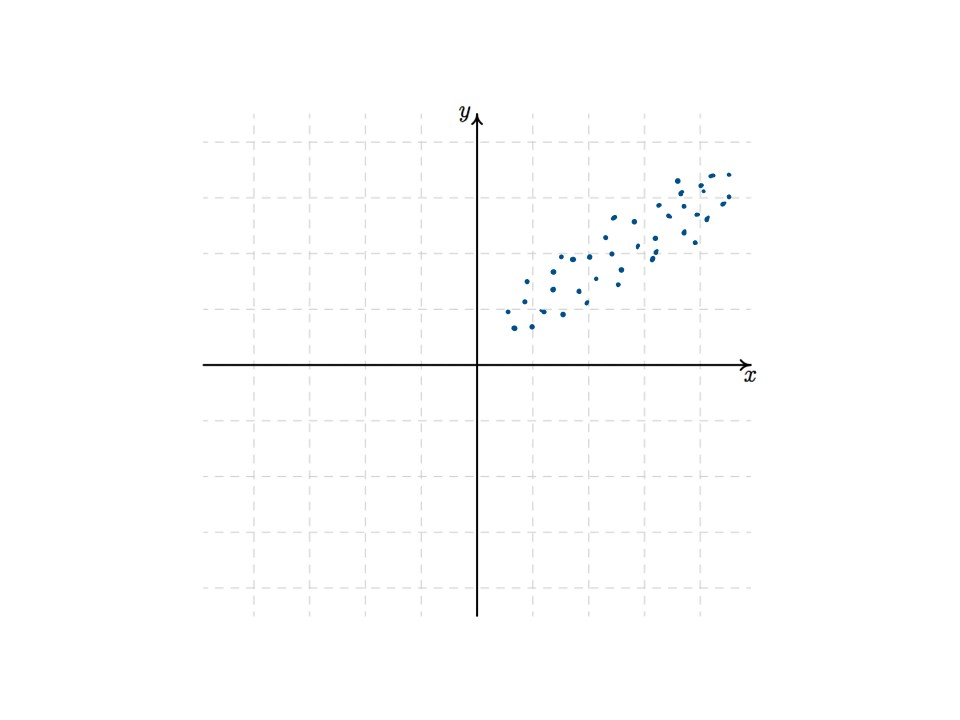
\includegraphics[width = 12 cm]{c and a.JPG}
\end{center}
}

\pagebreak

\easysubproblem{Give an example of two variables that are not correlated but are associated by drawing a plot.
\begin{center}
    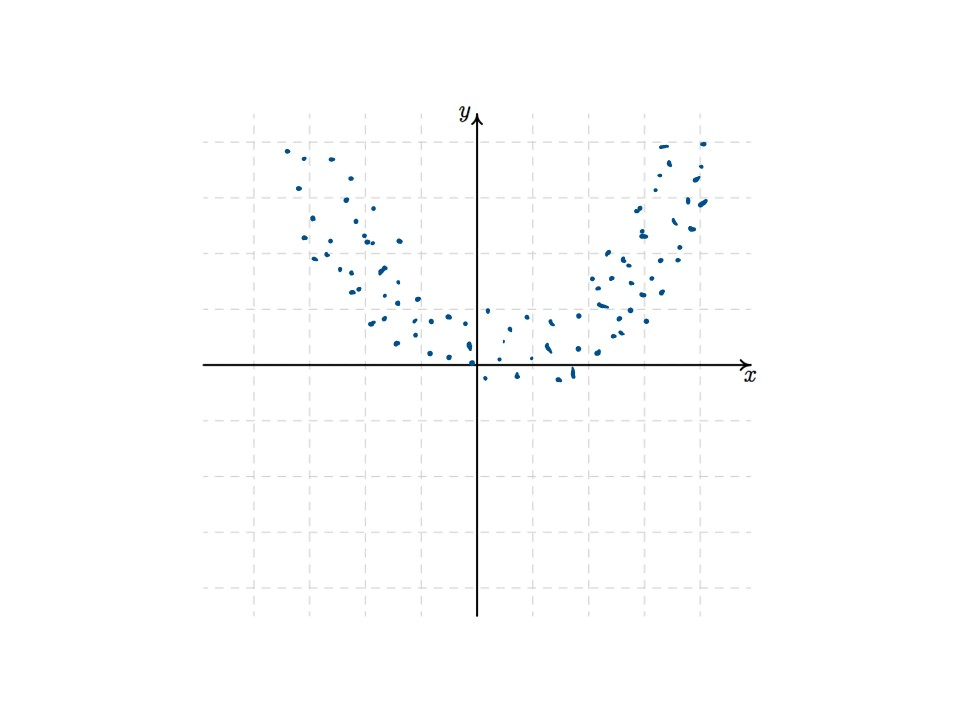
\includegraphics[width = 12 cm]{a not c.JPG}
\end{center}
}

\easysubproblem{Give an example of two variables that are not correlated nor associated by drawing a plot.
\begin{center}
    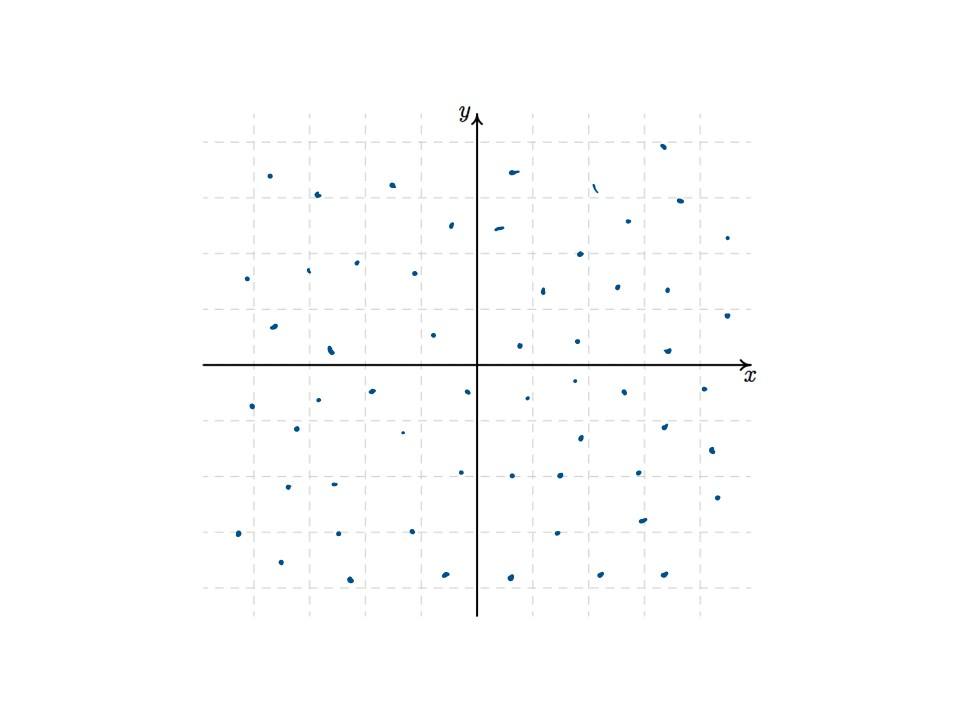
\includegraphics[width = 12 cm]{not a not c.JPG}
\end{center}
}

\easysubproblem{Can two variables be correlated but not associated? Explain.
\ans No. Since correlation is a measure of linear association, two variables must be linearly associated if they are correlated.
}

\hardsubproblem{[MA] Prove association $\centernot\implies$ correlation. This requires some probability theory.}\spc{5}

\end{enumerate}


\end{document}

\pagebreak
We want to prove $\XtX$ is invertible only when $\rank{\X} = p + 1$ i.e. the design matrix is \qu{full rank}. This is equivalent to proving that 

\beqn
\rank{\X} = p + 1 \implies \rank{\XtX} = p + 1
\eeqn

Logically equivalent is the contrapositive:

\beqn
\rank{\XtX} \neq p + 1 \implies \rank{\X} \neq p + 1
\eeqn

Not equal in this case is equivalent to less than because a matrix cannot have a rank that exceeds its number of columns since $\rank{\X} := \dim{\colsp{\X}}$ so the above is equivalent to:

\beqn
\rank{\XtX} < p + 1 \implies \rank{\X} < p + 1
\eeqn

Beginning with the premise on the left hand side, a rank-deficient matrix has at least one non-trivial (i.e. non-zero) vector $\v \in \reals^{p+1}$ that maps to the zero vector, i.e. there is at least one direction in the nullspace:

\beqn
\XtX\v = \bv{0}_{p+1}
\eeqn

Saqib noticed we can multiply both sides on the right by $\v^\top$ to arrive at:


\beqn
\v^\top\XtX\v = \v^\top\bv{0}_{p+1} = 0
\eeqn

We can write this alternatively as

\beqn
 (\X\v)^\top \X\v = 0 \implies \sum_{i=1}^n (\X\v)_i^2 = 0
\eeqn

If all elements of $\X\v$ squared and summed yield zero, every single element must be zero and thus,

\beqn
\X\v = \bv{0}_n
\eeqn

indicating that the vector $\v$ (which was assumed to be nontrivial above) is in the nullspace of $\X$ indicating that $\X$ is rank deficient and thus $\rank{\X} < p + 1.~ \blacksquare$ \pagestyle{empty}
